\documentclass[border=10pt]{standalone}
\usepackage{pgfplots}
\pgfplotsset{compat=1.18}
\usepackage{xcolor}
\begin{document}
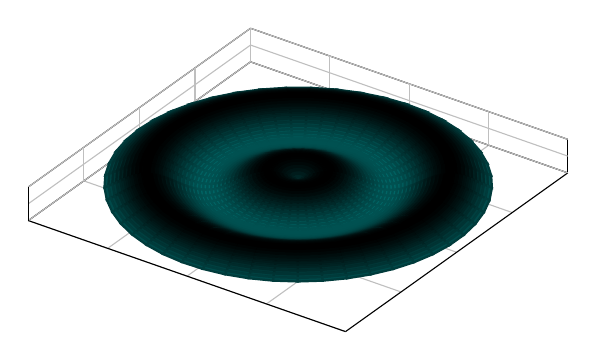
\begin{tikzpicture}
\begin{axis}[
  axis equal image, ticks=none,
  view={35}{30}, grid=major,
  zmin = -2, zmax = 2,
  domain     = -pi:pi,
  y domain   = 0:20,
  samples    = 50,
  samples y  = 50,
  colormap   = {tealblack}{color(0cm) = (teal!80!black); color(1cm) = (black)},
]
  \addplot3[
    surf, z buffer = sort,
    trig format plots = rad,
    line width=0.8pt
  ]
    ( {y*cos(x)},
      {y*sin(x)},
      {sin(0.5*y)}
    );
\end{axis}
\end{tikzpicture}
\end{document}